\documentclass[aspectratio=169,10pt]{beamer}
\usetheme{Madrid}
\usecolortheme{default}
\usepackage{tikz}
\usepackage{booktabs}
\usepackage{fontawesome5}
\usepackage{xcolor}
\usepackage{amsmath}
\usepackage{colortbl}
\usepackage{multirow}
\usepackage{listings}
\usepackage[most]{tcolorbox}
\usetikzlibrary{arrows.meta,shadows,positioning,fit,shapes.geometric,calc}

\lstdefinestyle{ccode}{
  language=C,
  basicstyle=\ttfamily\scriptsize,
  keywordstyle=\color{c1}\bfseries,
  commentstyle=\color{hit!80!black}\itshape,
  breaklines=true,
  showstringspaces=false,
  tabsize=2,
}

% ── palette ──────────────────────────────────────────────────────────
\definecolor{c1}{RGB}{41,128,185}
\definecolor{c2}{RGB}{52,152,219}
\definecolor{c3}{RGB}{155,89,182}
\definecolor{c4}{RGB}{142,68,173}
\definecolor{c5}{RGB}{230,126,34}
\definecolor{c6}{RGB}{211,84,0}
\definecolor{hit}{RGB}{39,174,96}
\definecolor{miss}{RGB}{192,57,43}
\definecolor{warn}{RGB}{243,156,18}

\setbeamercolor{frametitle}{bg=c1,fg=white}
\setbeamercolor{title}{fg=white}
\setbeamercolor{structure}{fg=c1}
\setbeamertemplate{navigation symbols}{}
\setbeamertemplate{footline}[frame number]
\setbeamerfont{frametitle}{series=\bfseries}

\newcommand{\chit}[1]{\cellcolor{hit!30} #1}
\newcommand{\cmiss}[1]{\cellcolor{miss!25} #1}
\newcommand{\cwarn}[1]{\cellcolor{warn!30} #1}
\newcommand{\czero}{\cellcolor{black!4} }


\title{Retrieval-Augmented Vulnerability Detection via Code Property Graphs}
\subtitle{From Graph-Based Patterns to Knowledge-Base Ranking}
\author{}
\date{May 2026}

\begin{document}

% =====================================================================
% TITLE SLIDE
% =====================================================================
\begin{frame}
  \titlepage
\end{frame}

% =====================================================================
% VULNERABILITY DEFINITION + CODE (progressive build)
% =====================================================================

% --- Slide 1: Definition + Code (no highlights) ---
\begin{frame}[fragile]{What Is a Vulnerability?}
  \begin{columns}
    \column{0.45\textwidth}
    \begin{tcolorbox}[colback=c1!5, colframe=c1!60!black, boxrule=0.6pt,
      left=6pt, right=6pt, top=6pt, bottom=6pt, arc=3pt, title={\scriptsize\bfseries NIST SP 800-53 / CWE Definition}]
      \small
      A \textbf{vulnerability} is a weakness in a system that can be exploited by a threat to gain unauthorized access or cause harm.
    \end{tcolorbox}

    \vspace{0.4cm}
    \textbf{Example:}\\
    % \textit{CVE-2024-56605} — 
    % CWE-416: 
     Use-After-Free\\[0.2cm]
    \footnotesize The program references memory after it has been freed, leading to undefined behavior.

    \column{0.55\textwidth}
    \begin{tcolorbox}[colback=c1!3, colframe=c1!40!black, boxrule=0.5pt,
      left=4pt, right=4pt, top=4pt, bottom=4pt, arc=3pt,
      shadow={0.5mm}{-0.5mm}{0mm}{black!15}]
    \begin{lstlisting}[style=ccode, basicstyle=\ttfamily\scriptsize\color{black!80},
      keywordstyle=\color{c4}\bfseries, commentstyle=\color{c1!70!black}\itshape,
      stringstyle=\color{c6}]
struct sock *alloc_socket(
    struct socket *sock) {
  struct sock *sk;

  sk = sk_alloc();       // allocate

  sock->sk = sk;         // alias created

  if (!chan_create()) {
    sk_free(sk);         // free original
    return NULL;    // BUG: alias dangling!
  }
  return sk;
}
    \end{lstlisting}
    \end{tcolorbox}
  \end{columns}
\end{frame}

% --- Slide 2: Highlight step 1 — allocation ---
\begin{frame}[fragile]{Tracing the Vulnerability (1/4): Allocation}
  \begin{columns}
    \column{0.55\textwidth}
    \begin{tcolorbox}[colback=c1!3, colframe=c1!40!black, boxrule=0.5pt,
      left=4pt, right=4pt, top=4pt, bottom=4pt, arc=3pt,
      shadow={0.5mm}{-0.5mm}{0mm}{black!15}]
    \begin{lstlisting}[style=ccode, basicstyle=\ttfamily\scriptsize\color{black!80},
      keywordstyle=\color{c4}\bfseries, commentstyle=\color{c1!70!black}\itshape,
      stringstyle=\color{c6}, escapechar=@]
struct sock *alloc_socket(
    struct socket *sock) {
  struct sock *sk;

  @\colorbox{hit!30}{sk = sk\_alloc();}@       // allocate

  sock->sk = sk;         // alias created

  if (!chan_create()) {
    sk_free(sk);         // free original
    return NULL;
  }
  return sk;
}
    \end{lstlisting}
    \end{tcolorbox}

    \column{0.45\textwidth}
    \begin{enumerate}
      \item[\faCheckCircle] \textbf{\texttt{sk} is allocated} — a new object is created on the heap
    \end{enumerate}
  \end{columns}
\end{frame}

% --- Slide 3: Highlight step 2 — alias creation ---
\begin{frame}[fragile]{Tracing the Vulnerability (2/4): Alias Creation}
  \begin{columns}
    \column{0.55\textwidth}
    \begin{tcolorbox}[colback=c1!3, colframe=c1!40!black, boxrule=0.5pt,
      left=4pt, right=4pt, top=4pt, bottom=4pt, arc=3pt,
      shadow={0.5mm}{-0.5mm}{0mm}{black!15}]
    \begin{lstlisting}[style=ccode, basicstyle=\ttfamily\scriptsize\color{black!80},
      keywordstyle=\color{c4}\bfseries, commentstyle=\color{c1!70!black}\itshape,
      stringstyle=\color{c6}, escapechar=@]
struct sock *alloc_socket(
    struct socket *sock) {
  struct sock *sk;

  @\colorbox{hit!30}{sk = sk\_alloc();}@       // allocate

  @\colorbox{warn!30}{sock->sk = sk;}@         // alias created

  if (!chan_create()) {
    sk_free(sk);         // free original
    return NULL;
  }
  return sk;
}
    \end{lstlisting}
    \end{tcolorbox}

    \column{0.45\textwidth}
    \begin{enumerate}
      \item[\faCheckCircle] \texttt{sk} is allocated
      \item[\faCheckCircle] \textbf{\texttt{sock->sk} becomes an alias} — two pointers now reference the same object
    \end{enumerate}
  \end{columns}
\end{frame}

% --- Slide 4: Highlight step 3 — free ---
\begin{frame}[fragile]{Tracing the Vulnerability (3/4): Free}
  \begin{columns}
    \column{0.55\textwidth}
    \begin{tcolorbox}[colback=c1!3, colframe=c1!40!black, boxrule=0.5pt,
      left=4pt, right=4pt, top=4pt, bottom=4pt, arc=3pt,
      shadow={0.5mm}{-0.5mm}{0mm}{black!15}]
    \begin{lstlisting}[style=ccode, basicstyle=\ttfamily\scriptsize\color{black!80},
      keywordstyle=\color{c4}\bfseries, commentstyle=\color{c1!70!black}\itshape,
      stringstyle=\color{c6}, escapechar=@]
struct sock *alloc_socket(
    struct socket *sock) {
  struct sock *sk;

  @\colorbox{hit!30}{sk = sk\_alloc();}@       // allocate

  @\colorbox{warn!30}{sock->sk = sk;}@         // alias created

  if (!chan_create()) {
    @\colorbox{miss!25}{sk\_free(sk);}@         // free original
    return NULL;
  }
  return sk;
}
    \end{lstlisting}
    \end{tcolorbox}

    \column{0.45\textwidth}
    \begin{enumerate}
      \item[\faCheckCircle] \texttt{sk} is allocated
      \item[\faCheckCircle] \texttt{sock->sk} becomes an alias
      \item[\faCheckCircle] \textbf{On error, \texttt{sk} is freed} — the object is deallocated
    \end{enumerate}
  \end{columns}
\end{frame}

% --- Slide 5: Highlight step 4 — dangling pointer (the bug) ---
\begin{frame}[fragile]{Tracing the Vulnerability (4/4): Dangling Pointer}
  \begin{columns}
    \column{0.55\textwidth}
    \begin{tcolorbox}[colback=c1!3, colframe=c1!40!black, boxrule=0.5pt,
      left=4pt, right=4pt, top=4pt, bottom=4pt, arc=3pt,
      shadow={0.5mm}{-0.5mm}{0mm}{black!15}]
    \begin{lstlisting}[style=ccode, basicstyle=\ttfamily\scriptsize\color{black!80},
      keywordstyle=\color{c4}\bfseries, commentstyle=\color{c1!70!black}\itshape,
      stringstyle=\color{c6}, escapechar=@]
struct sock *alloc_socket(
    struct socket *sock) {
  struct sock *sk;

  @\colorbox{hit!30}{sk = sk\_alloc();}@       // allocate

  @\colorbox{warn!30}{sock->sk = sk;}@         // alias created

  if (!chan_create()) {
    @\colorbox{miss!25}{sk\_free(sk);}@         // free original
    @\colorbox{miss!25}{return NULL;}@    // BUG: alias dangling!
  }
  return sk;
}
    \end{lstlisting}
    \end{tcolorbox}

    \column{0.45\textwidth}
    \begin{enumerate}
      \item[\faCheckCircle] \texttt{sk} is allocated
      \item[\faCheckCircle] \texttt{sock->sk} becomes an alias
      \item[\faCheckCircle] On error, \texttt{sk} is freed
      \item[\textcolor{red}{\faBug}] \textbf{\texttt{sock->sk} still points to freed memory!}
    \end{enumerate}

    \vspace{0.5cm}
    \textbf{Pattern:}\\
    Free without nullifying all aliases\\
    $\Rightarrow$ \textcolor{red}{\textbf{Use-After-Free}}

    \vspace{0.3cm}
    \footnotesize\textit{Key insight: this pattern leaves a structural fingerprint in the code graph.}
  \end{columns}
\end{frame}




% =====================================================================
% CPG VISUALIZATION — Overview (raw Joern output)
% =====================================================================
\begin{frame}{Code Property Graph: Full Joern Output}
  \begin{columns}
    \column{0.3\textwidth}
    \centering
    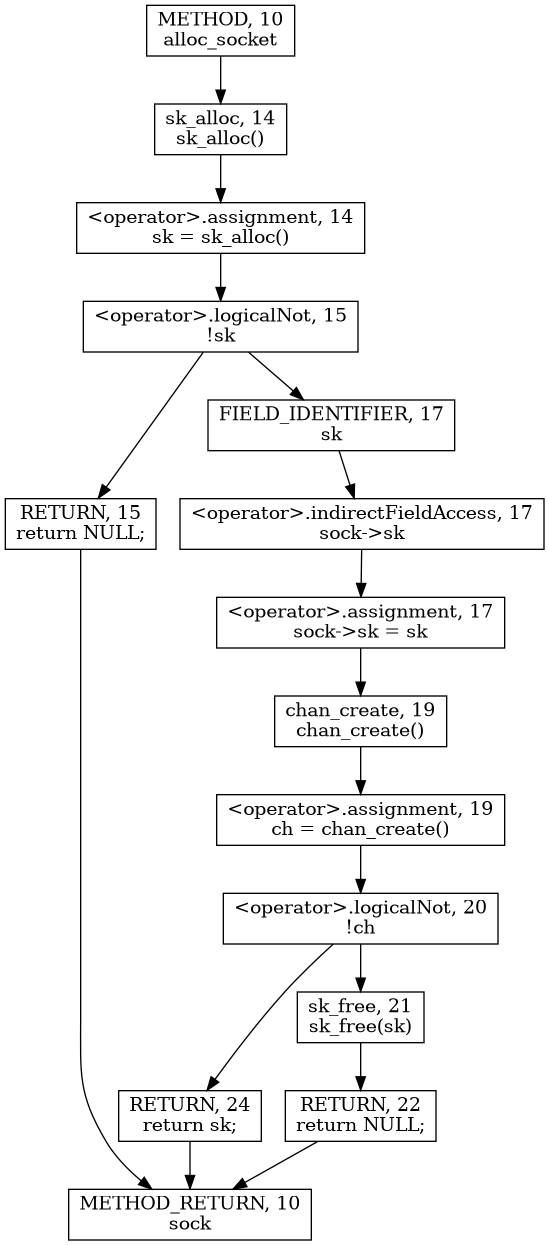
\includegraphics[width=0.75\textwidth]{joern_cfg_raw.png}
    \column{0.45\textwidth}
    \textbf{What the CPG encodes:}
    \begin{itemize}
      \item \textbf{AST} — syntax structure
      \item \textbf{CFG} — execution order
      \item \textbf{DDG} — data flow (def $\to$ use)
      \item \textbf{CDG} — control dependencies
    \end{itemize}

    \vspace{0.3cm}
    \footnotesize
    Full graph is detailed — let's simplify to the vulnerability-relevant subgraph.
  \end{columns}
\end{frame}

% =====================================================================
% CPG VISUALIZATION — Simplified vulnerable vs. patched
% =====================================================================
\begin{frame}{Structure Reveals the Vulnerability}
  \begin{columns}
    % --- Vulnerable graph ---
    \column{0.48\textwidth}
    \centering
    \textbf{\textcolor{miss}{Vulnerable}}
    \vspace{0.2cm}

    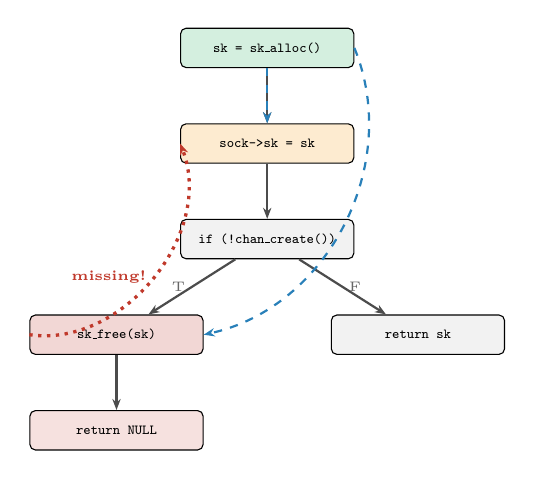
\begin{tikzpicture}[
      node distance=0.7cm,
      n/.style={draw, rounded corners=2pt, font=\tiny\ttfamily,
        minimum width=2.2cm, minimum height=0.5cm, align=center},
      cfg/.style={-{Stealth[length=4pt]}, thick, black!70},
      ddg/.style={-{Stealth[length=4pt]}, thick, c1, dashed},
      every node/.append style={inner sep=2pt}
    ]
      \node[n, fill=hit!20] (alloc) {sk = sk\_alloc()};
      \node[n, fill=warn!20, below=of alloc] (alias) {sock->sk = sk};
      \node[n, fill=black!5, below=of alias] (branch) {if (!chan\_create())};
      \node[n, fill=miss!20, below left=0.7cm and -0.3cm of branch] (free) {sk\_free(sk)};
      \node[n, fill=black!5, below right=0.7cm and -0.3cm of branch] (ret) {return sk};
      \node[n, fill=miss!15, below=of free] (retnull) {return NULL};

      % CFG edges
      \draw[cfg] (alloc) -- (alias);
      \draw[cfg] (alias) -- (branch);
      \draw[cfg] (branch) -- node[left, font=\tiny, text=black!60]{T} (free);
      \draw[cfg] (branch) -- node[right, font=\tiny, text=black!60]{F} (ret);
      \draw[cfg] (free) -- (retnull);

      % DDG edges
      \draw[ddg] (alloc) -- (alias);
      \draw[ddg] (alloc.east) to[bend left=50] (free.east);

      % Missing edge annotation
      \draw[miss, very thick, dotted, -{Stealth[length=4pt]}]
        (free.west) to[bend right=60]
        node[left, font=\tiny\bfseries, text=miss]{missing!} (alias.west);
    \end{tikzpicture}

    \vspace{0.2cm}
    \footnotesize\textcolor{miss}{No nullification of alias after free}

    % --- Patched graph ---
    \column{0.48\textwidth}
    \centering
    \textbf{\textcolor{hit}{Patched}}
    \vspace{0.2cm}

    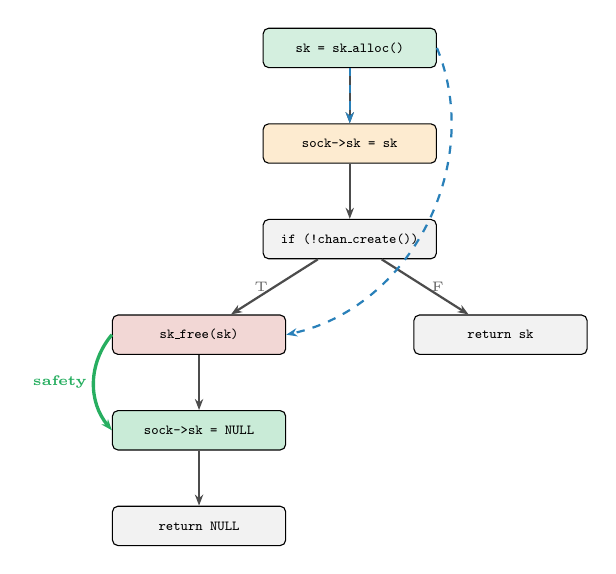
\begin{tikzpicture}[
      node distance=0.7cm,
      n/.style={draw, rounded corners=2pt, font=\tiny\ttfamily,
        minimum width=2.2cm, minimum height=0.5cm, align=center},
      cfg/.style={-{Stealth[length=4pt]}, thick, black!70},
      ddg/.style={-{Stealth[length=4pt]}, thick, c1, dashed},
      every node/.append style={inner sep=2pt}
    ]
      \node[n, fill=hit!20] (alloc) {sk = sk\_alloc()};
      \node[n, fill=warn!20, below=of alloc] (alias) {sock->sk = sk};
      \node[n, fill=black!5, below=of alias] (branch) {if (!chan\_create())};
      \node[n, fill=miss!20, below left=0.7cm and -0.3cm of branch] (free) {sk\_free(sk)};
      \node[n, fill=black!5, below right=0.7cm and -0.3cm of branch] (ret) {return sk};
      \node[n, fill=hit!25, below=of free] (null) {sock->sk = NULL};
      \node[n, fill=black!5, below=of null] (retnull) {return NULL};

      % CFG edges
      \draw[cfg] (alloc) -- (alias);
      \draw[cfg] (alias) -- (branch);
      \draw[cfg] (branch) -- node[left, font=\tiny, text=black!60]{T} (free);
      \draw[cfg] (branch) -- node[right, font=\tiny, text=black!60]{F} (ret);
      \draw[cfg] (free) -- (null);
      \draw[cfg] (null) -- (retnull);

      % DDG edges
      \draw[ddg] (alloc) -- (alias);
      \draw[ddg] (alloc.east) to[bend left=50] (free.east);

      % Safety edge
      \draw[hit, very thick, -{Stealth[length=4pt]}]
        (free.west) to[bend right=40]
        node[left, font=\tiny\bfseries, text=hit]{safety} (null.west);
    \end{tikzpicture}

    \vspace{0.2cm}
    \footnotesize\textcolor{hit}{Alias nullified $\Rightarrow$ no dangling pointer}
  \end{columns}

  \vspace{0.4cm}
  \begin{center}
    \small
    \textbf{Takeaway:} The \emph{structural difference} between vulnerable and patched code is a single edge/node.\\[0.15cm]
    Vulnerabilities leave fingerprints in the graph — prior work (Yamaguchi et al., 2014 — \textit{Joern}) exploits this for detection.
  \end{center}
\end{frame}


% =====================================================================
% MOTIVATION: PRIOR WORK LIMITATIONS
% =====================================================================
\begin{frame}{Motivation: Why Not Just Train a Graph Classifier?}
  
    \textbf{Prior work exploits the same insight} — code structure reveals vulnerabilities:
    \begin{itemize}
      \item Train GNNs / graph kernels on labeled CPGs or PDGs
      \item Learn to classify subgraphs as vulnerable vs.\ safe
      \item Devign, ReVeal, IVDetect, \ldots
    \end{itemize}
    
    \vspace{0.5cm}
    \textbf{But these approaches hit a wall:}
    \begin{itemize}
      \item Require large labeled datasets (expensive to curate)
      \item Struggle to generalize to \emph{unseen} vulnerability types
      \item Treat each vulnerability independently — no knowledge reuse
    \end{itemize}
    
    \vspace{0.5cm}
    \textbf{Our alternative:} Instead of \emph{classifying}, \textbf{retrieve}.\\
    Store known vulnerability patterns as graph embeddings in a knowledge base,\\
    then rank new code by structural similarity — no retraining needed.
    
  %   \column{0.5\textwidth}
  %   \textbf{Our Insight:}
  %   \begin{itemize}
  %     \item Leverage KB of known patterns
  %     \item Focus on ranking/precision, not detection
  %     \item Works with limited training data
  %   \end{itemize}
    
  %   \vspace{0.5cm}
  %   \textbf{Key Question:}
  %   \begin{itemize}
  %     \item Can structural embeddings rival semantic models?
  %     \item How to rank vulnerability patterns?
  %     \item Does it generalize to real code?
  %   \end{itemize}
  % \end{columns}
\end{frame}

% =====================================================================
% PROPOSAL OVERVIEW
% =====================================================================
\begin{frame}[fragile]{System Architecture: Graph-RAG Pipeline}
  \begin{center}
  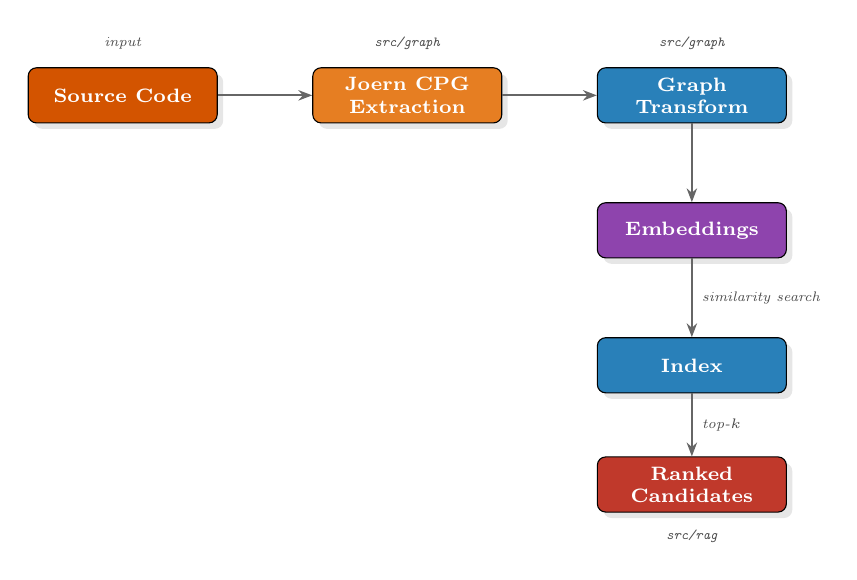
\begin{tikzpicture}[
    node distance=0.6cm and 1.2cm,
    box/.style={draw, rounded corners=3pt, minimum height=0.7cm,
      minimum width=2.4cm, font=\scriptsize\bfseries, align=center,
      fill=#1, text=white, drop shadow={opacity=0.2}},
    box/.default=c1,
    arrow/.style={-{Stealth[length=5pt]}, thick, color=black!60},
    label/.style={font=\tiny\itshape, text=black!70}
  ]
    % Row 1: Input
    \node[box=c6] (source) {Source Code};
    \node[box=c5, right=of source] (joern) {Joern CPG\\Extraction};
    \node[box=c1, right=of joern] (graph) {Graph\\Transform};

    % Row 2: Embeddings
    \node[box=c4, below=1cm of graph] (embed) {Embeddings};
    

    % Row 3: Retrieval
    \node[box=c1, below=1cm of embed] (index) {Index};

    % Row 4: Output
    \node[box=miss, below=0.8cm of index] (rank) {Ranked\\Candidates};

    % Arrows
    \draw[arrow] (source) -- (joern);
    \draw[arrow] (joern) -- (graph);
    \draw[arrow] (graph) -- (embed);
    \draw[arrow] (embed) -- node[label, right]{similarity search} (index);
    \draw[arrow] (index) -- node[label, right]{top-$k$} (rank);

    % Labels
    \node[label, above=0.1cm of source] {input};
    \node[label, above=0.1cm of joern] {\texttt{src/graph}};
    \node[label, above=0.1cm of graph] {\texttt{src/graph}};
    \node[label, below=0.1cm of rank] {\texttt{src/rag}};
  \end{tikzpicture}
  \end{center}
\end{frame}

\begin{frame}{}
    Feasibility (AutoPatch dataset, n=225):
    used AutoPatch as a controlled dataset to validate the concept and define baselines
    baselines: structure-only embeddings (NetLSD + WL + GIN combined) vs. CodeBERT
    result: comparable retrieval performance between CodeBERT and combined structural embeddings
        → structural graph representations capture vulnerability patterns as effectively as pretrained code models

    
    
  \vspace{1cm}
  \begin{center}
    \textbf{Hypothesis:} Structural graph representations are as effective as semantic code models for vulnerability pattern matching, and KB-guided ranking improves precision on complex real-world vulnerabilities.
  \end{center}
\end{frame}

% =====================================================================
% PHASE 1: AUTOPATCH RESULTS
% =====================================================================
\begin{frame}{Phase 1: Feasibility — AutoPatch Dataset (n=225)}
  \textbf{Goal:} Validate that structural embeddings match CodeBERT performance.

  \vspace{0.3cm}
  \begin{table}
    \centering
    \tiny
    \begin{tabular}{lrrrr}
      \toprule
      \textbf{Embedder} & \textbf{H@1} & \textbf{H@5} & \textbf{MRR} & \textbf{CWE R.} \\
      \midrule
      \multicolumn{5}{c}{\textit{Structure-Only}} \\
      \midrule
      Combined & 0.8904 & 0.9589 & 0.9162 & 0.4978 \\
      GIN & 0.7260 & 0.8767 & 0.7879 & 0.4427 \\
      WL & 0.6986 & 0.7945 & 0.7363 & 0.4386 \\
      NetLSD & 0.3288 & 0.5479 & 0.4172 & 0.2096 \\
      \midrule
      \multicolumn{5}{c}{\textit{CodeBERT (Baseline)}} \\
      \midrule
      CodeBERT (seq) & 0.7534 & 0.8630 & 0.7927 & 0.4121 \\
      CodeBERT (pat) & 0.7123 & 0.8356 & 0.7677 & 0.4147 \\
      \bottomrule
    \end{tabular}
  \end{table}

  \vspace{0.3cm}
  \textbf{Key Finding:} Combined structural embeddings (89\% Hit@1) outperform CodeBERT (75\%).
\end{frame}

% =====================================================================
% PHASE 2: CVEFIXES RESULTS
% =====================================================================
\begin{frame}{Phase 2: Generalization — CVEfixes Dataset}
  \textbf{Question:} Does the approach generalize to real-world vulnerabilities?
   \textbf{Generalization} — Test on real-world complex code (CVEfixes)
  \vspace{0.3cm}
  \begin{table}
    \centering
    \tiny
    \begin{tabular}{lrrrr}
      \toprule
      \textbf{Embedder} & \textbf{H@1} & \textbf{H@5} & \textbf{MRR} & \textbf{CWE R.} \\
      \midrule
      \multicolumn{5}{c}{\textit{Structure-Only (n=74 index, 20 query)}} \\
      \midrule
      Combined & 0.1176 & 0.1176 & 0.1176 & 0.2367 \\
      GIN & 0.0000 & 0.0588 & 0.0196 & 0.2383 \\
      \midrule
      \multicolumn{5}{c}{\textit{CodeBERT (Baseline)}} \\
      \midrule
      CodeBERT (pat) & 0.1176 & 0.1176 & 0.1176 & 0.2367 \\
      \bottomrule
    \end{tabular}
  \end{table}

  \vspace{0.3cm}
  \textbf{The Generalization Gap:} Performance drops from 0.8904 to 0.1176 (10\% of Phase 1).
  
  \vspace{0.3cm}
  \textbf{Root Causes:}
  \begin{itemize}
    \item Shallow code slicing (depth-1) loses critical context
    \item Inter-procedural aliasing not captured
    \item CVEfixes code far more complex than AutoPatch
  \end{itemize}
\end{frame}

% =====================================================================
% PHASE 3: PROPOSED DIRECTION
% =====================================================================
\begin{frame}{Phase 3: Candidate Sink Ranking via KB-Guided Retrieval}
  
\end{frame}


% =====================================================================
% CHALLENGES
% =====================================================================
\begin{frame}{Why This Matters: The Challenge of Precision}
  \textbf{Challenge 1: False Positives from Static Analysis}
  \begin{itemize}
    \item Joern finds: \textit{``free() without alias nullification''}
    \item But not all are real UAF (e.g., no caller accesses the alias)
    \item Joern has \textbf{high recall, low precision}
  \end{itemize}

  \vspace{0.5cm}
  \textbf{Challenge 2: Context Sensitivity}
  \begin{itemize}
    \item Alias creation hidden behind function calls
    \item Inter-procedural data flow crucial
    \item Single-function analysis insufficient
  \end{itemize}

  % \vspace{0.5cm}
  % \textbf{Our Solution: Knowledge-Base Ranking}
  % \begin{itemize}
  %   \item \textbf{Joern:} Generate candidates (high recall)
  %   \item \textbf{KB Retrieval:} Rank by similarity to known vulnerability graphs
  %   \item \textbf{Result:} Filter FP, focus on true patterns
  % \end{itemize}

  \vspace{0.5cm}
  \begin{center}
    \textcolor{blue}{Together: high recall \textbf{+} high precision}
  \end{center}
\end{frame}

% =====================================================================
% SUMMARY
% =====================================================================
\begin{frame}{Summary: From Feasibility to Precision}
 
\end{frame}

% =====================================================================
% BACKUP: DETAILED CPG
% =====================================================================
\begin{frame}{Appendix: CPG Deep Dive}
  The Code Property Graph encodes four types of relationships:

  \vspace{0.5cm}
  \begin{description}
    \item[AST:] Abstract syntax tree (structure of code)
    \item[CFG:] Control flow graph (which statements execute in sequence)
    \item[DDG:] Data dependency graph (variable definitions and uses)
    \item[CDG:] Control dependency graph (which statements depend on conditionals)
  \end{description}

  \vspace{0.5cm}
  \textbf{For vulnerability detection:}
  \begin{itemize}
    \item Look for patterns in DDG (data flow anomalies)
    \item Combine with CFG to understand execution order
    \item Use CDG to understand conditional branches (e.g., error handling)
  \end{itemize}

  \vspace{0.5cm}
  Joern exposes all four via traversals; KB retrieval compares the combined structure to find similar vulnerabilities.
\end{frame}

% =====================================================================
% JOERN QUERY
% =====================================================================
\begin{frame}[fragile]{Joern Query: Finding the Pattern}
  \textbf{Goal:} Find \texttt{free()} calls with dangling aliases.

  \vspace{0.15cm}
  \tiny
  \begin{verbatim}
val uafCandidates = cpg.call.name(".*free.*")
  .map { freeCall =>
    val freedVar = freeCall.argument(1).code
    val aliases = freeCall.method.assignment
      .where(_.source.isIdentifier.name(freedVar))
      .target.code.l
    val freeLineNo = freeCall.lineNumber.get
    val nullified = freeCall.method.assignment
      .where(_.lineNumber.map(_ > freeLineNo))
      .target.code.l
    val dangling = aliases.filterNot(nullified.contains)
    (freeCall, dangling)
  }
  \end{verbatim}

  \normalsize
  \textbf{Output:} \texttt{[UAF] sk\_free(sk) — dangling: sock->sk}
\end{frame}



\end{document}
